\providecommand{\main}{../../../..}
\documentclass[\main/dresen_thesis.tex]{subfiles}
\begin{document}
  \label{sec:doublelayers:layers:pnr}
  Write something
  % \begin{figure}[tb]
  %   \centering
  %   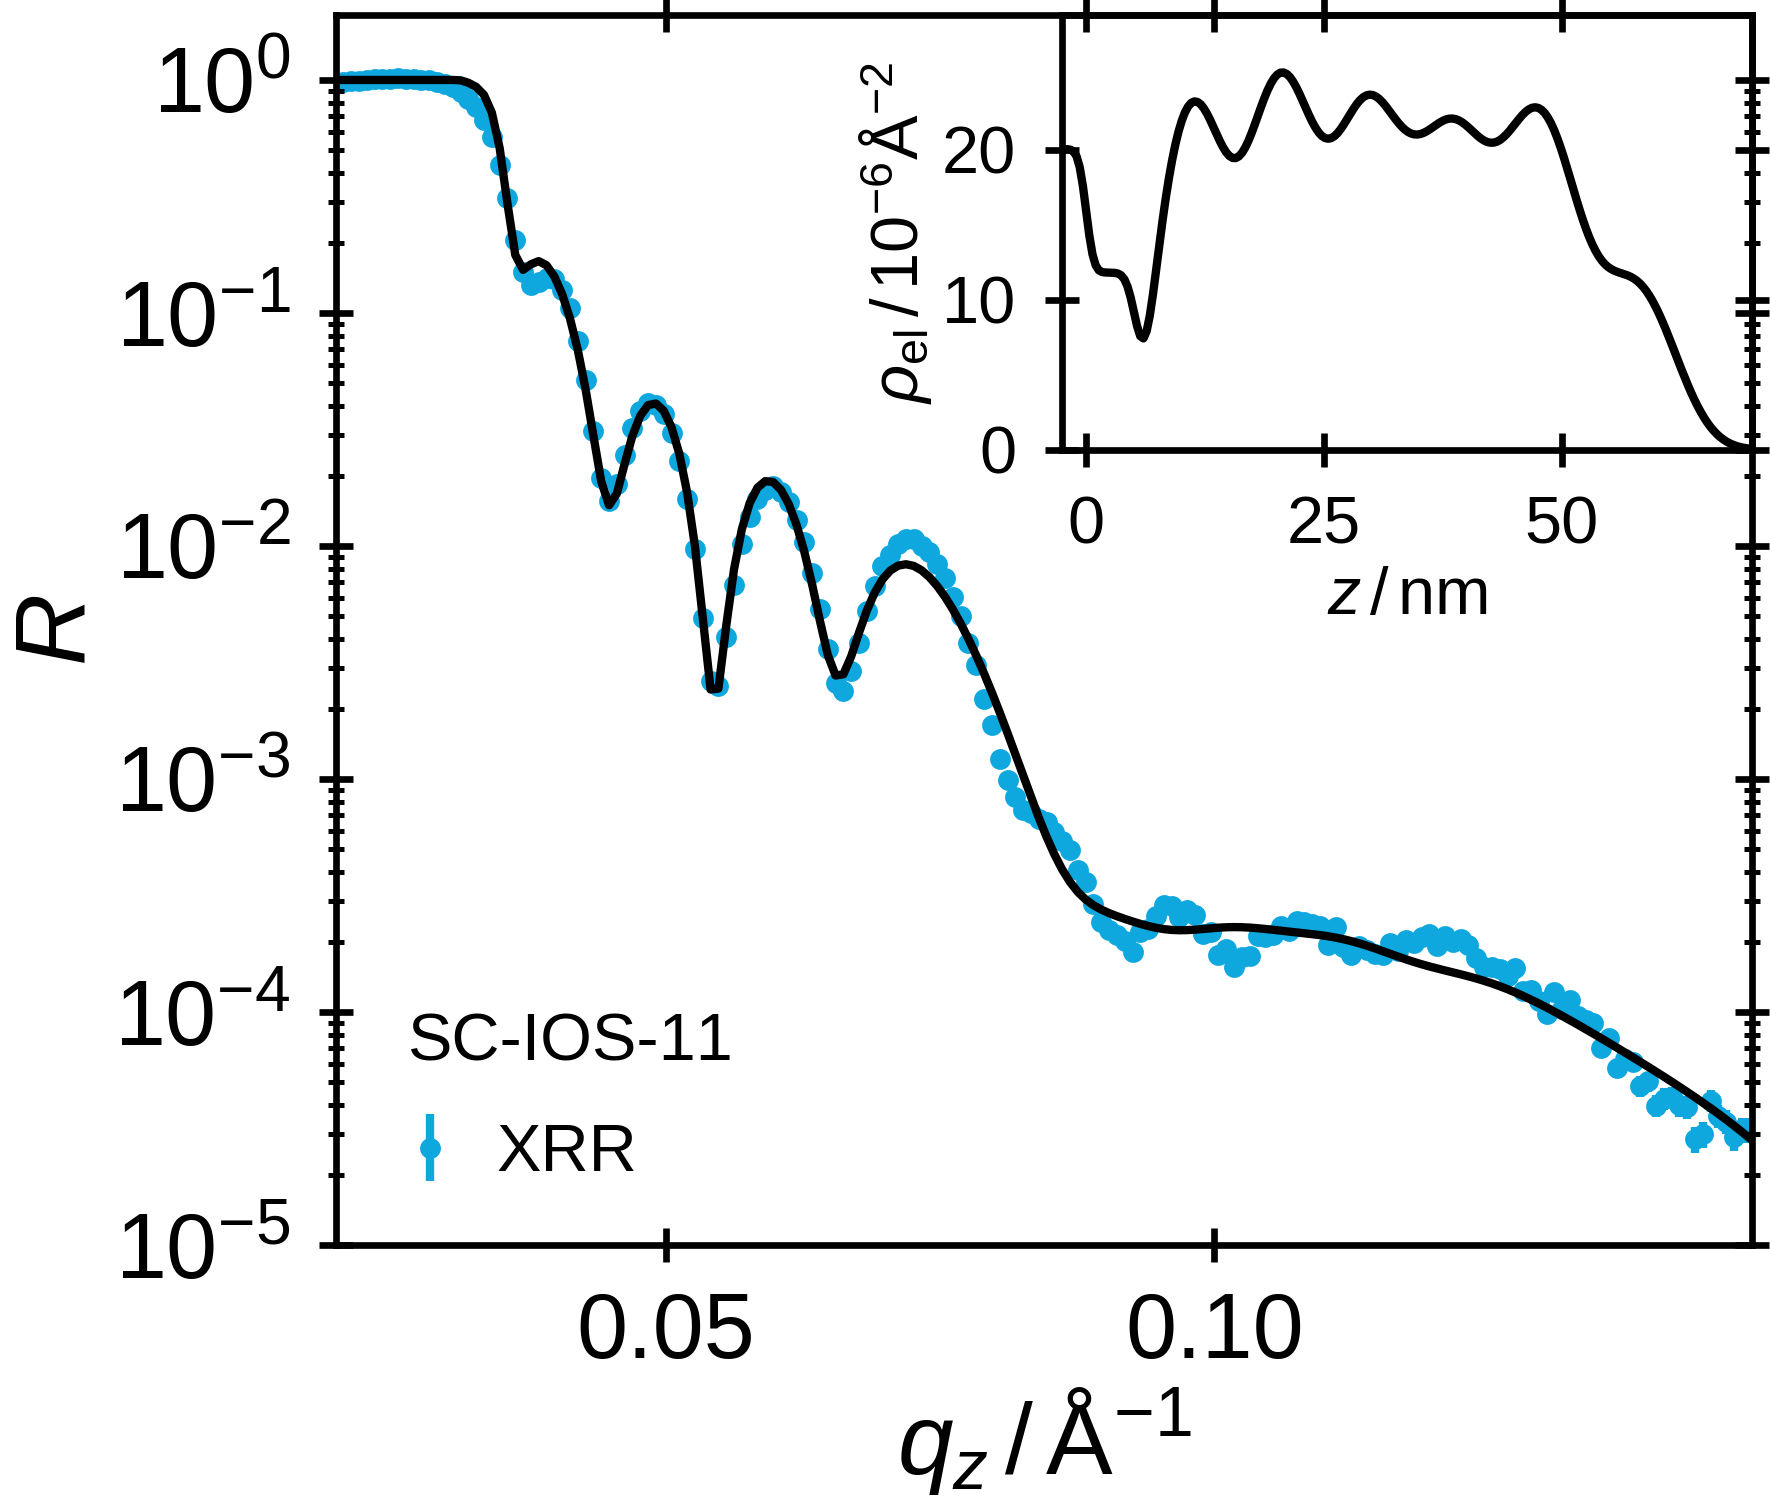
\includegraphics{looselyPackedNP_VerticalStructure_SC-IOS-11_XRR}
  %   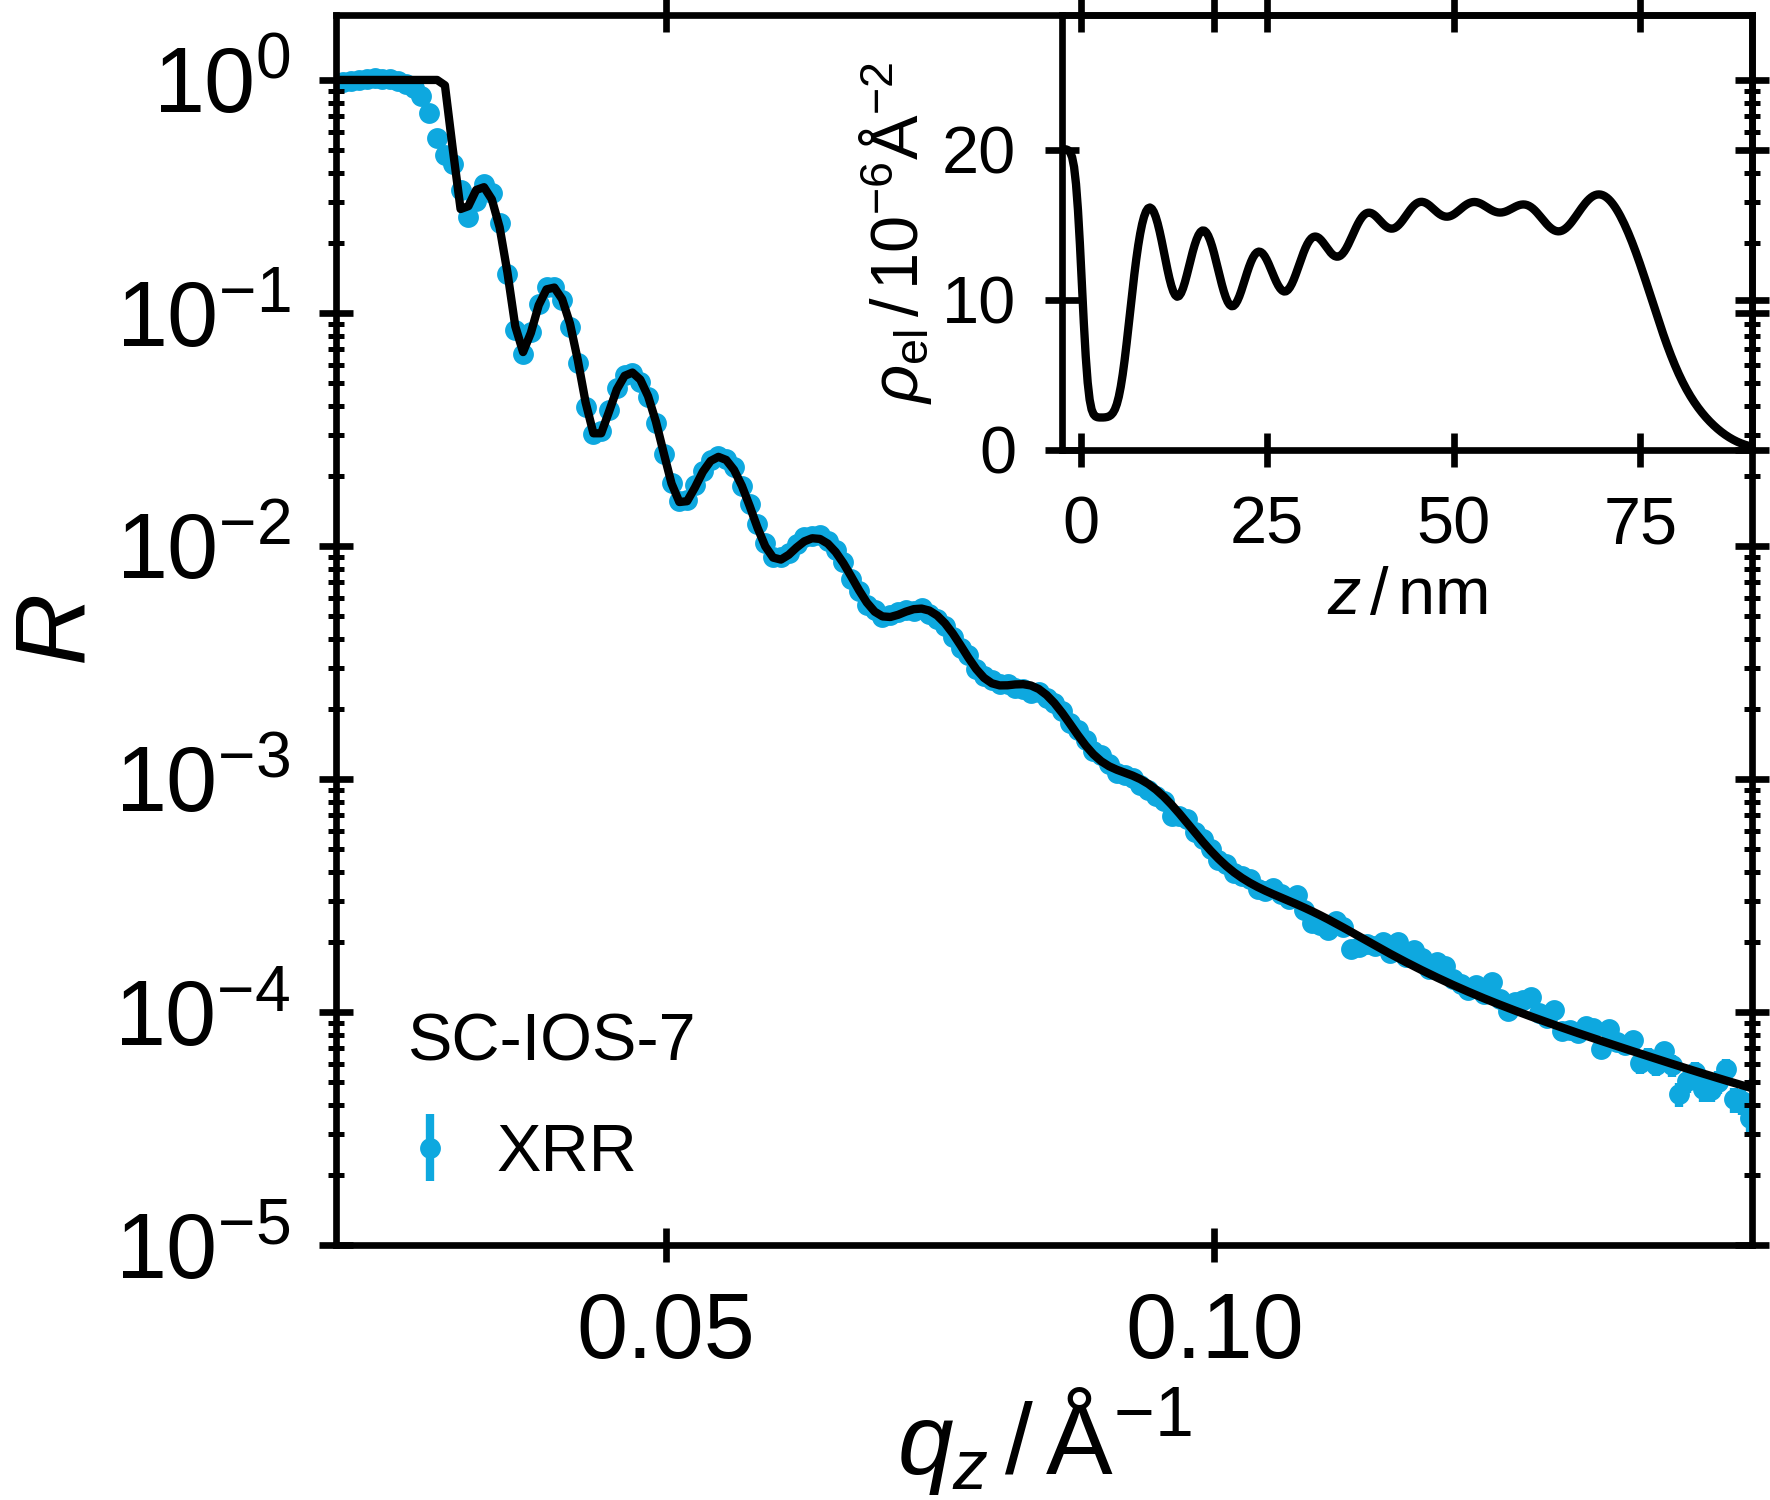
\includegraphics{looselyPackedNP_VerticalStructure_SC-IOS-7_XRR}
  %   \caption{\label{fig:looselyPackedNP:layer:xrr}X-ray reflectometry from SC-IOS-11 (left) and SC-IOS-7 (right). The inset shows the scattering length density model of the fitted reflectometry curve (black).}
  % \end{figure}

  % The depth-resolved average electron density of the layers SC-IOS-11 and SC-IOS-7 is resolved with sub-nm precision using X-ray reflectometry measured on a Bruker D8 Advance.
  % The observed reflectivity is shown in \reffig{fig:looselyPackedNP:layer:xrr}, where a footprint correction has been applied with an equidistributed beam profile.
  % The reflectivity is fit by assuming that the sample is compromised of multiple stacked spheres, which rest on a silicon substrate.
  % The separate sphere layers are allowed each to have a variable two dimensional packing $\eta_i$ and their position can be shifted by $\Delta z_i$ from the ideal position that is calculated for the spheres if they had a hard oleic acid shell and do not penetrate each other.
  % The determined parameters for each layer are tabulated in \reftab{tab:looselyPackedNP:nanoparticle:xrr} for both IOS-11 and IOS-7.

  % \begin{table}[!htbp]
  %   \centering
  %   \caption{\label{tab:looselyPackedNP:nanoparticle:xrr}Parameters for the layer of multiple nanospheres shown in \reffig{fig:looselyPackedNP:layer:xrr}. The parameters $\eta$ are the two dimensional packing density for each layer and $\Delta z$ are the shifts of the layer center from the pitch $\sqrt{8/3} (R+D_\mathrm{OA}$). The other parameters are the thickness of the spacer layer on the substrate $d_\mathrm{spacer}$, its SLD $\rho_\mathrm{spacer}$, the substrate roughness $\sigma$, the rate of roughness increase with layer height $\Delta \sigma$, and the wavelength spread of the instrument $\sigma_\lambda / \lambda$. The nanosphere parameters are fixed from SAXS.}
  %   \begin{tabular}{ c | l | l }
  %     \rule{0pt}{2ex} \textbf{XRR}  & \textbf{SC-IOS-11} & \textbf{SC-IOS-7} \\
  %     \hline
  %      $\eta_1     \, / \unit{\%}$                                  & $50.9(4)$         & $34(1)$    \\
  %      $\eta_2     \, / \unit{\%}$                                  & $55.4(4)$         & $32(1)$    \\
  %      $\eta_3     \, / \unit{\%}$                                  & $52.9(5)$         & $30(2)$    \\
  %      $\eta_4     \, / \unit{\%}$                                  & $49.8(6)$         & $33(3)$    \\
  %      $\eta_5     \, / \unit{\%}$                                  & $53.4(8)$         & $38(3)$    \\
  %      $\eta_6     \, / \unit{\%}$                                  & $28.6(1.0)$       & $40(3)$    \\
  %      $\eta_7     \, / \unit{\%}$                                  &                   & $41(3)$    \\
  %      $\eta_8     \, / \unit{\%}$                                  &                   & $44(3)$    \\
  %      $\eta_9     \, / \unit{\%}$                                  &                   & $43(7)$    \\
  %      $\eta_{10}     \, / \unit{\%}$                               &                   & $34(9)$    \\
  %      $\eta_{11}     \, / \unit{\%}$                               &                   & $8(10)$    \\
  %      \hline
  %      $\Delta z_1 \, / \unit{nm} $                                 & $-1.04(3)$        & $-1.33(6)$ \\
  %      $\Delta z_2 \, / \unit{nm} $                                 & $-2.60(3)$        & $-1.33(7)$ \\
  %      $\Delta z_3 \, / \unit{nm} $                                 & $-2.68(3)$        & $-1.13(8)$ \\
  %      $\Delta z_4 \, / \unit{nm} $                                 & $-2.95(4)$        & $-1.22(6)$ \\
  %      $\Delta z_5 \, / \unit{nm} $                                 & $-2.67(4)$        & $-1.40(6)$ \\
  %      $\Delta z_6 \, / \unit{nm} $                                 & $-1.82(10)$       & $-1.46(7)$ \\
  %      $\Delta z_7 \, / \unit{nm} $                                 &                   & $-1.41(9)$ \\
  %      $\Delta z_8 \, / \unit{nm} $                                 &                   & $-1.2(1)$   \\
  %      $\Delta z_9 \, / \unit{nm} $                                 &                   & $-0.4(5)$    \\
  %      $\Delta z_{10} \, / \unit{nm} $                              &                   & $-2.4(8)$   \\
  %      $\Delta z_{11} \, / \unit{nm} $                              &                   & $-1.5(19)$  \\
  %      \hline
  %      $d_\mathrm{spacer}   \, / \unit{nm} $                        & $5.15(3)$         & $5.27(2)$  \\
  %      $\rho_\mathrm{spacer}\, / \unit{10^{-6} \angstrom^{-2}} $    & $11.9(2)$         & $2.2(1)$ \\
  %      $\sigma     \, / \unit{nm} $                                 & $0.65(1)$         & $0.70(1)$  \\
  %      $\Delta \sigma$                                              & $0.034(1)$        & $0.036(1)$ \\
  %      $\sigma_\lambda / \lambda\, / \unit{\%}$                     & \multicolumn{2}{c}{$1.1(2)$} \\
  %     \hline
  %      $R             \, / \unit{nm}$                               & $5.41$         & $3.54$ \\
  %      $D_\mathrm{OA} \, / \unit{nm}$                               & $1.82$         & $1.69$ \\
  %      $\sigma_R      \, / \unit{\%}$                               & $5.45$         & $7.52$ \\
  %      $\rho_\mathrm{core}\, / \unit{10^{-6} \angstrom^{-2}}      $ & \multicolumn{2}{c}{$40.5$}\\
  %      $\rho_\mathrm{shell}\, / \unit{10^{-6} \angstrom^{-2}}     $ & \multicolumn{2}{c}{$8.52$}\\
  %      $\rho_\mathrm{substrate}\, / \unit{10^{-6} \angstrom^{-2}} $ & \multicolumn{2}{c}{$20.1$}\\
  %     \hline
  %   \end{tabular}
  % \end{table}

  % The illustrative model is able to describe the characteristics of the two obtained reflectivity curves for most parts.
  % The SLD profile of SC-IOS-11 shows five layers of nanospheres with an additional sixth layer of decreased packing fraction.
  % The two dimensional packing fractions $\eta$ are in the order of $50 \unit{\%}$ for the five layers and $29 \unit{\%}$ for the upper layer.
  % $\Delta z$ is in all cases negative in the order of $1 - 3 \unit{nm}$.
  % For SC-IOS-7 the same observation in $\Delta z$ can be made with a lesser degree of inter-mixing as the values are in the order of $1 - 1.5 \unit{nm}$.
  % Furthermore in the case of SC-IOS-7 the packing fraction $\eta$ are lower being in an order of magnitude of $30 - 40 \unit{\%}$.
  % The spacer thickness is in both cases approximately $5 \unit{nm}$ and the additional roughness parameter in an order of $0.7 \unit{nm}$ at the substrate.
  % In both cases, the roughness increases with a slope of $0.035$ with respect to the layer height, yielding a roughness of approximately $2.5 \unit{nm}$ near the sample surface.

  % The fitted roughness parameter is to be understood in this context as a model of the spread in the respective layer positions across the measured area within the reflectivity experiment.
  % The increasing roughness with layer height is therefore to be understood as a larger uncertainty in the positions of the specific layer across the sample.

  % The parameters, excluding the roughness, are used to generate the depiction of the sphere stacking shown in \reffig{fig:looselyPackedNP:layer:xrrDepiction}.
  % Here, the two-dimensional packing fraction $\eta$ are translated into an average particle distance in the layer by
  % \begin{align}
  %   r_\mathrm{pp} \eq \sqrt{\frac{\eta_\mathrm{CP}}{\eta}} 2 (R + D_\mathrm{OA}),
  % \end{align}
  % where $\eta_\mathrm{CP}$ is the dense circle packing fraction given by $\eta_\mathrm{CP} \eq \pi / \sqrt{12} \approx 90.7 \%$.
  % From the depiction it becomes visible for IOS-SC-11 that the shift down from the calculated pitch correlates with the lowered lateral packing density as the spheres fill the voids.
  % Additionally it is visible that the oleic acid shells of stacked particles overlap to some part.
  % For IOS-SC-7 the particles are more spaced relative to each other and the density of the packing increases from the lower to the higher parts of the layer slightly.

  % \begin{figure}[tb]
  %   \centering
  %   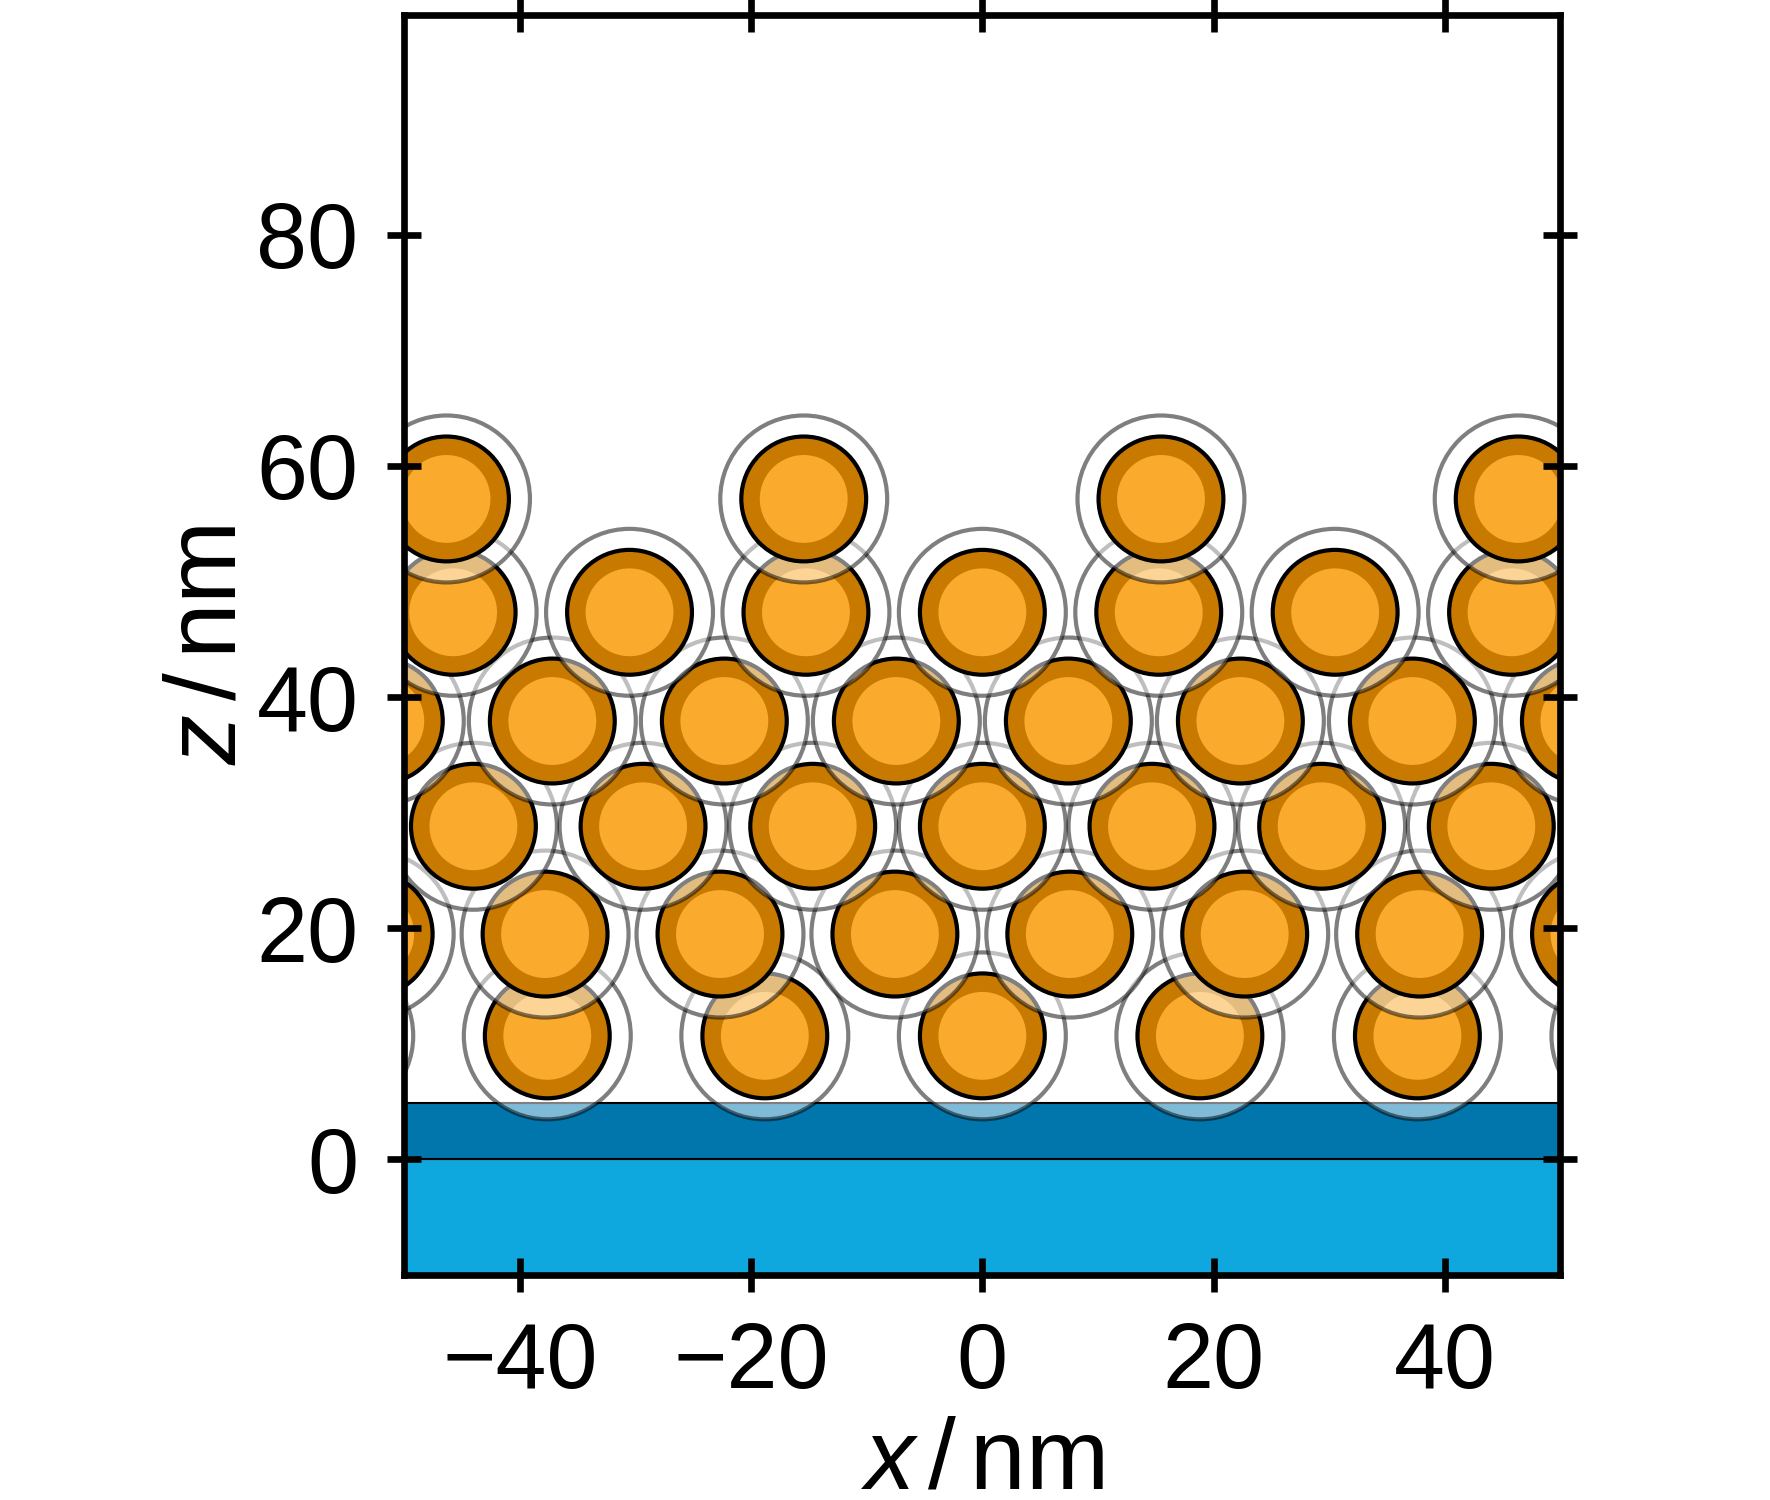
\includegraphics{looselyPackedNP_VerticalStructure_SC-IOS-11_XRRDepiction}
  %   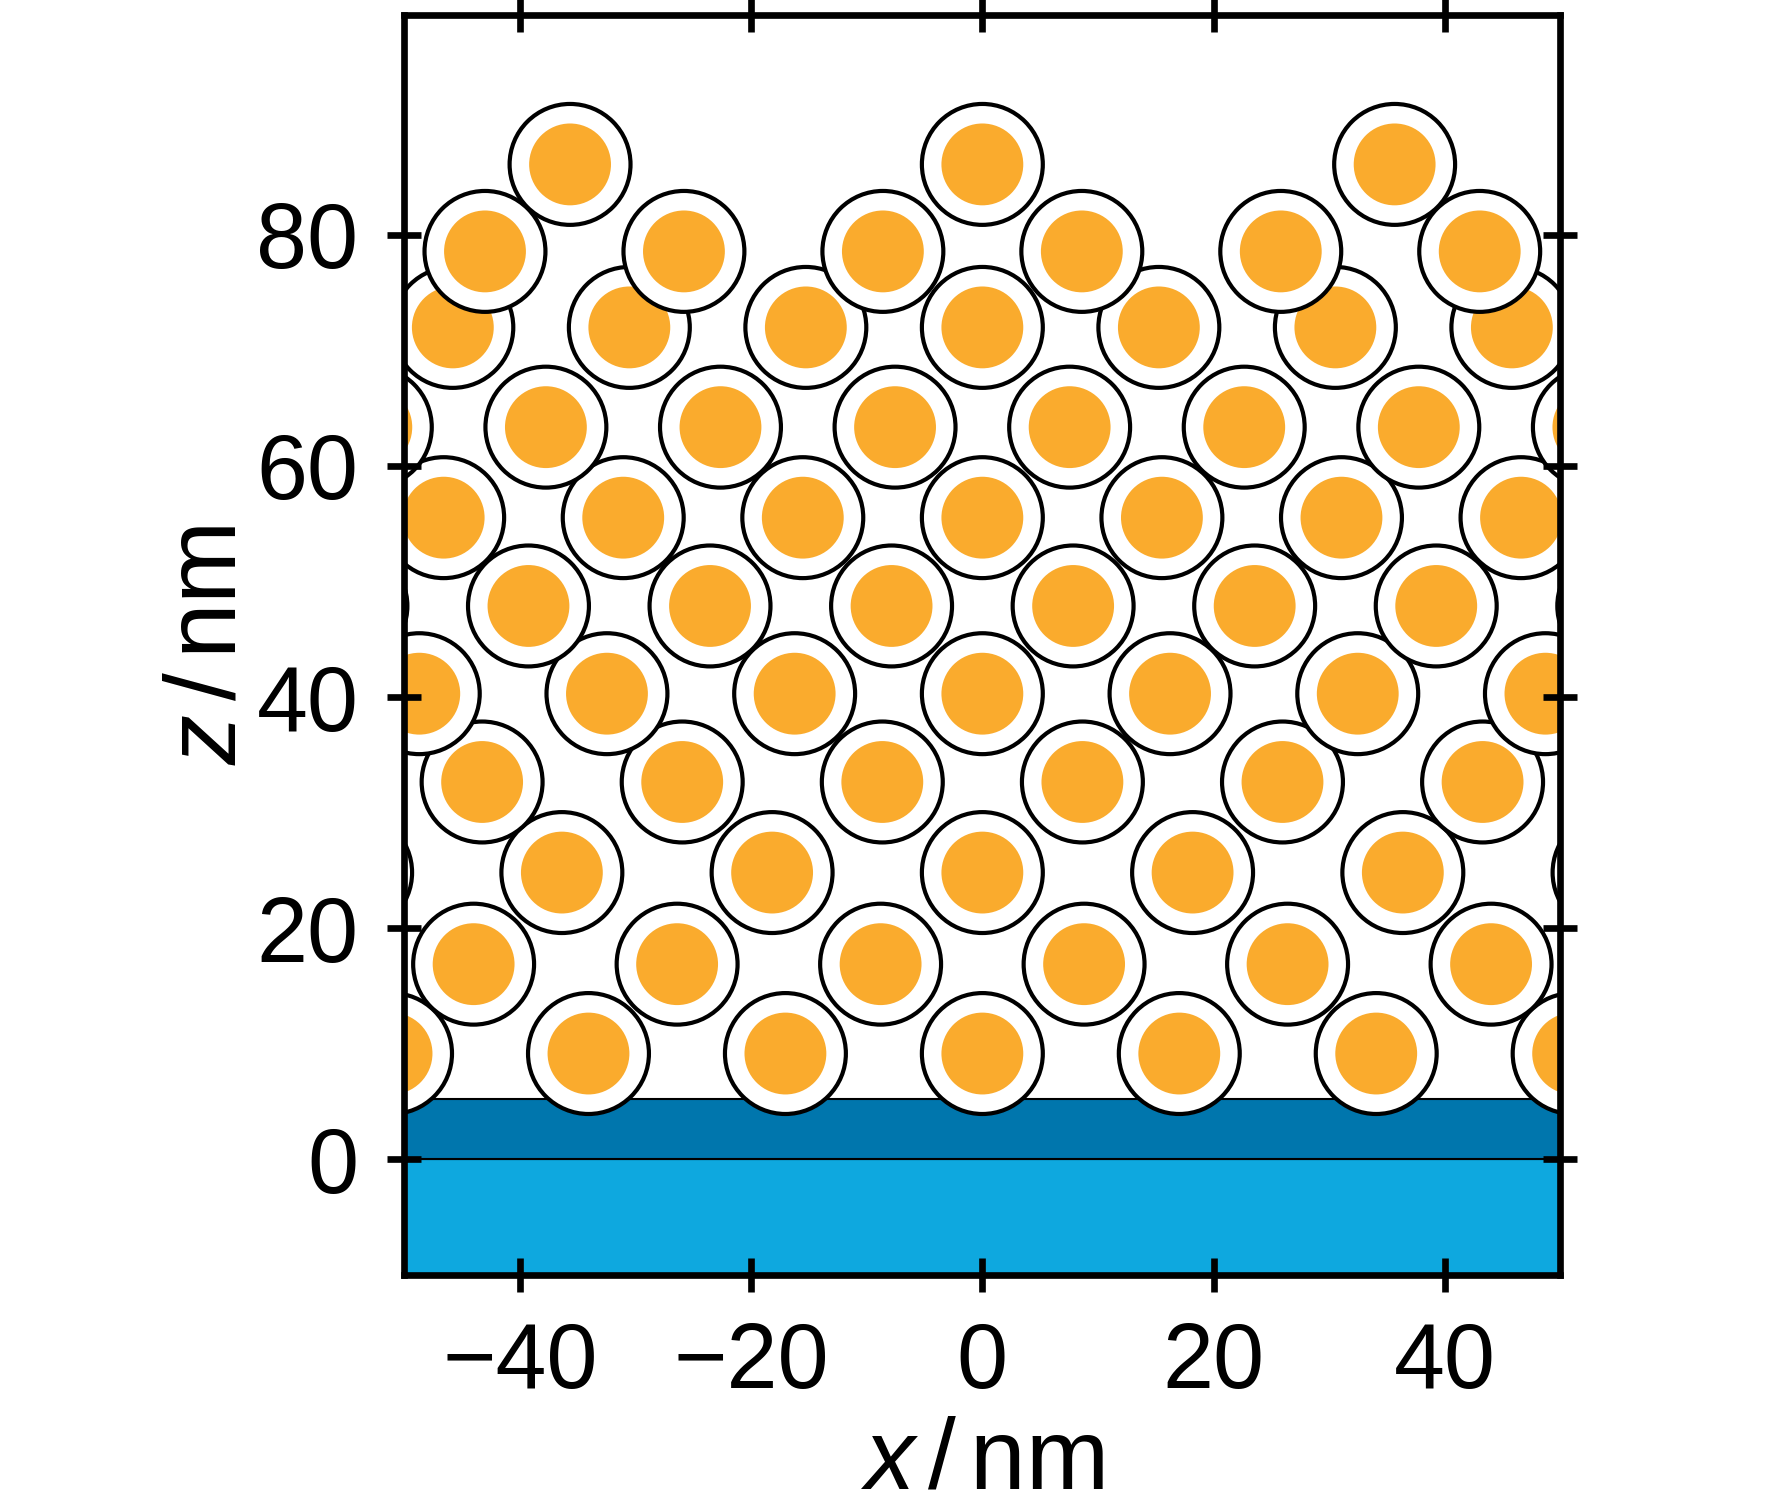
\includegraphics{looselyPackedNP_VerticalStructure_SC-IOS-7_XRRDepiction}
  %   \caption{\label{fig:looselyPackedNP:layer:xrrDepiction}Depiction generated from the fitted parameters in \reftab{tab:looselyPackedNP:nanoparticle:xrr} showing the average particle distance and layer packing.}
  % \end{figure}

\end{document}